\chapter{Managing and Understanding the Boot Procedure}
\section{Boot Procedure Generic Overview}
On starting up, the computer perform a "Power On Self Test" (POST). During this, the computer checks all the connected hardware and finds the boot device, which is typically a hard disk / solid state drive (HDD/SSD). On the boot device, the computer access Grub 2, the boot loader, that loads the \textbf{kernel} and \textbf{initrd}. 

\begin{figure}[H]
	\centering
	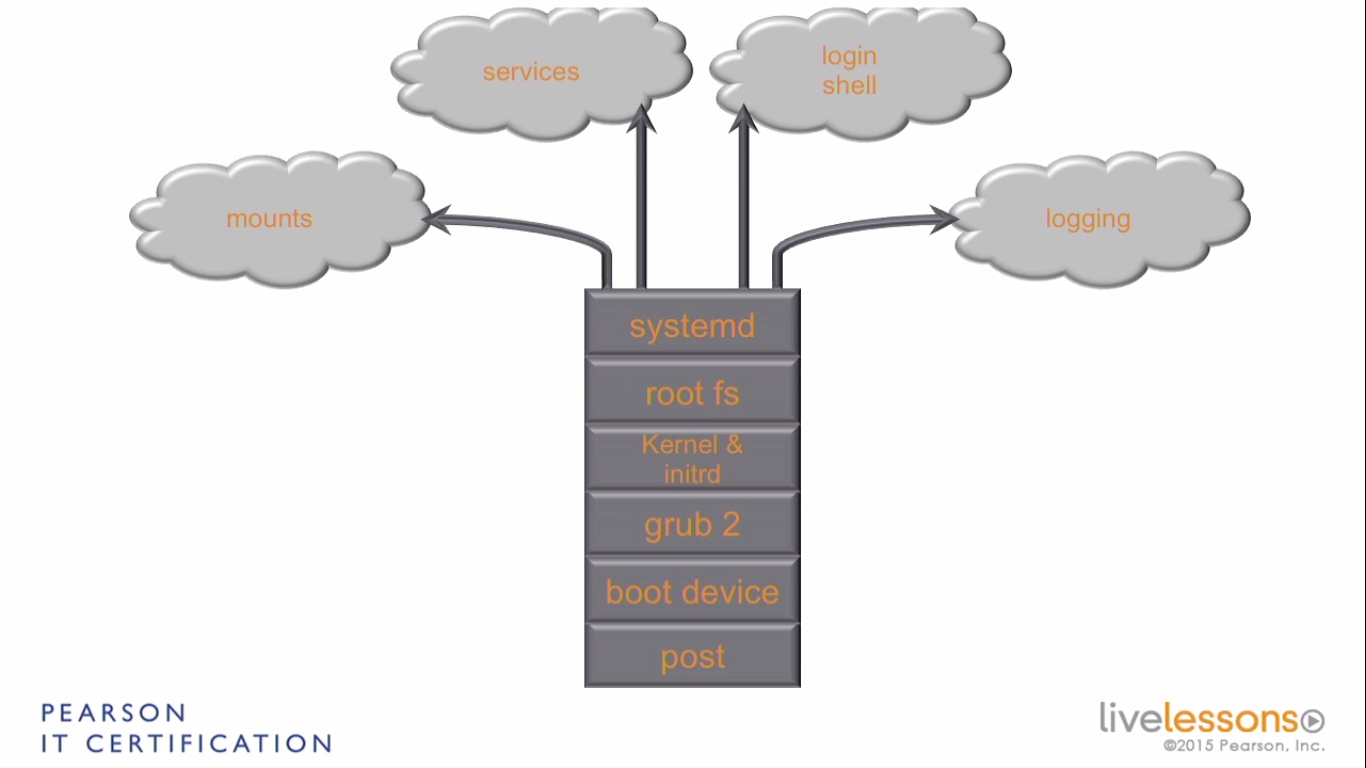
\includegraphics[width=0.9\linewidth]{RHCSA/Mod3/chapters/3.19.a}
	\caption{Boot Procedure}
	\label{fig:3 Boot Procedure}
\end{figure}

Next, the root file system is mounted (by the kernel) and then, \textbf{systemd} is started. Once systemd has started, everything else can begin, such as: logging, mounting the other file systems, starting all services and preparing the login shell. 

\section{Understanding Grub2}
The very first thing from the linux perspective (i.e., the first thing that's executed) when a computer boots is Grub2 (Grand Unified Boot-loader). 

The \verb|/etc/default/grub| is the most important configuration file for Grub2. Most of the customizations/modifications by an user is done to this file. There are also additional configuration files in the \verb|/etc/grub.d| directory. If any of the configuration files have been updated, the boot loader needs to be updated as well, by using the \verb|grub2-mkconfig| command. This updates the data in the Master Boot Record (MBR) and the metadata in the first few sectors of our hard drives. 

Once the computer boots, we can access the Grub boot menu by pressing the \textit{escape} key. When this is done, we can enter special boot instructions on it.

\subsection{Booting in emergency mode}
On the boot menu, we need to enter \verb|systemd.unit=emergency.target| as a boot option to start up the computer in emergency mode, which is used in case the computer can't boot normally. 

The diagram below explains the entire boot procedure. Once the power is supplied to the computer, it performs the Power On Self Test and then loads the boot loader from the MBR. Now, we have the option to enter the boot menu by pressing the escape key, and enter the boot options, like booting in emergency mode. 

\begin{figure}[H]
	\centering
	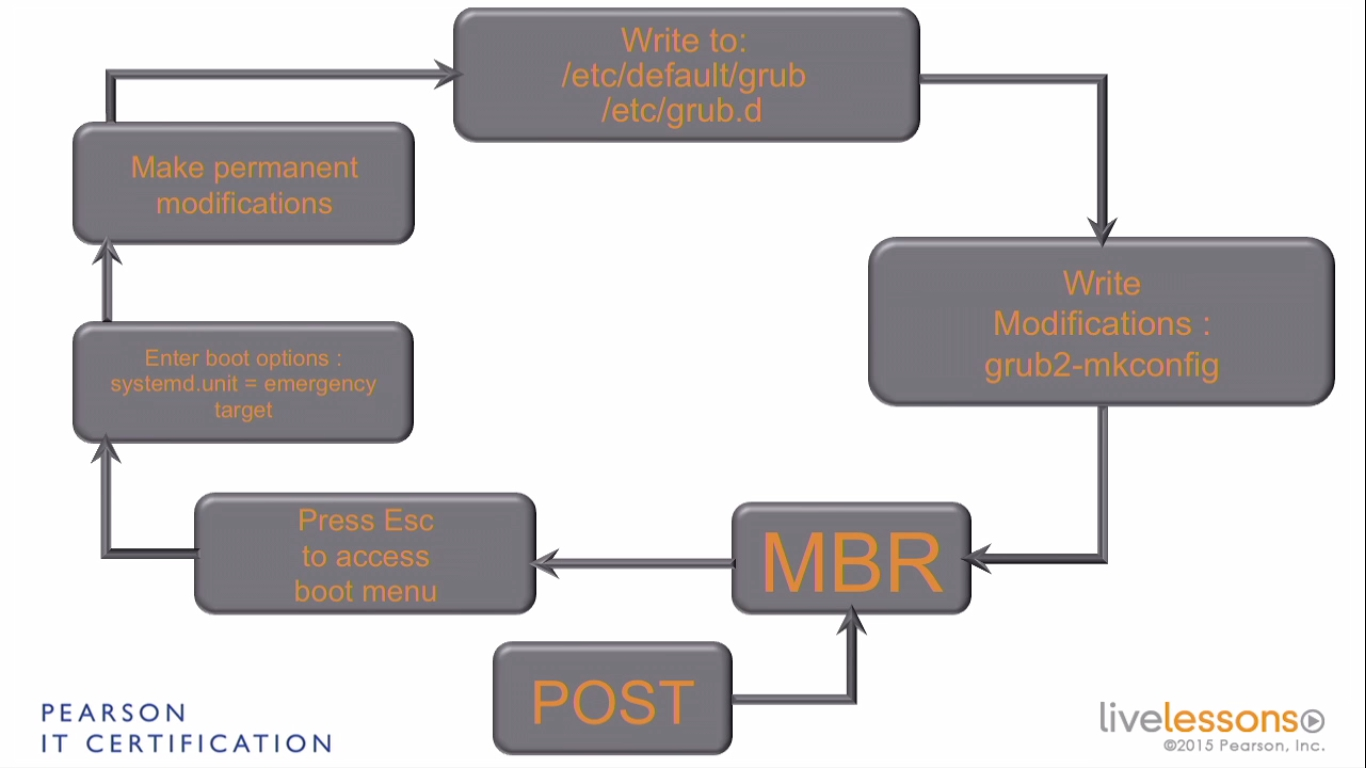
\includegraphics[width=0.9\linewidth]{RHCSA/Mod3/chapters/3.19.b}
	\caption{Booting in emergency mode}
	\label{fig:3 Booting in emergency mode}
\end{figure}

\noindent
In case there's something wrong with the bootloader itself, we can make permanent modifications by editing the files: \verb|/etc/default/grub| and the config files in \verb|/etc/grub.d| directory. Once these modifications have been written, the boot loader needs to be updated using \verb|grub2-mkconfig| command. This ensures that the next time the MBR will be read, the edited grub2 configuration files will be used. 

	\section{Modifying Grub2 Parameters}
The primary grub configuration file is \verb|/etc/default/grub|. The default contents of it look like:

\vspace{-15pt}
\begin{minted}{bash}
GRUB_TIMEOUT=5
GRUB_DISTRIBUTOR="$(sed 's, release .*$,,g' /etc/system-release)"
GRUB_DEFAULT=saved
GRUB_DISABLE_SUBMENU=true
GRUB_TERMINAL_OUTPUT="console"
GRUB_CMDLINE_LINUX="crashkernel=auto rd.lvm.lv=centos/root rd.lvm.lv=centos/swap rhgb quiet"
GRUB_DISABLE_RECOVERY="true"
\end{minted}
\vspace{-10pt}

\noindent
The \verb|GRUB_TIMEOUT| parameter defines the amount of time the system waits in the Grub boot menu for user input. The most important parameter is \verb|GRUB_CMDLINE_LINUX| which defines which arguments are passed on to the linux kernel when the system is booting. The last portion of this parameter, \verb|rhgb quiet| stops Grub from showing us what it's doing during boot. To enable this feature, we need to delete those arguments. 

Next, we take a look at the \verb|/etc/grub.d| directory. The files in here are shell scripts that aren't meant to be changed normally, and help with the boot process. 

After making all changes, we need to execute the \verb|grub2-mkconfig| command to update the changes to the Grub2 boot-loader. The command reads (and compiles) every grub related config file. This generates a grub configuration file (to send to the boot loader). 

To see all these changes, we need to reboot our computer. To verify that the changes have been applied correctly, we can enter the Grub menu using the \textit{Escape} key. In there, we can find the kernel line with all the options that are used. A \textit{CTRL+X} at this point causes a reboot with the new parameters passed to the kernel. 

\section{Understanding Systemd}
\textbf{Systemd} is a major new feature added in RHEL 7. It is a new init system that starts things - it both bootstraps the current user-space as well as manage the system processes after booting. 

During startup, right after the loading of the kernel, systemd is started, and systemd in turn takes care of starting everything else. Unlike the older \textit{runlevel} system, where only services were started, systemd takes care of services, mounting partitions, auto mounting file systems, and much more. 

\subsection{Unit file}
A \textbf{unit} file is the replacement of the old init script. Init scripts were relatively more difficult to understand. The unit files have greater readability. 

This unit file defines how to start services and everything else systemd can do, as well as define the relation between all those things. Systemd has two different locations for the storing of scripts - the default scripts are stored in \verb|/usr/lib/systemd| and the administrator's custom scripts reside in the \verb|/etc/systemd| directory. 

\section{Managing Services in a systemd Environment}
To get a task done in Linux, we need services, which are started using systemd. The directory \verb|/usr/lib/systemd/system| contains many service scripts (among other files). This directory is for the default services that are installed by the RPMs. Thus, we shouldn't edit the files in this directory. 

For our own system service management needs, we go to the \verb|/etc/systemd/system| folder. This has two advantages: i) updates to the RPMs that dropped the service scripts in \verb|/usr/lib/systemd/system| won't overwrite our scripts, and ii) Our scripts in \verb|/etc/systemd/system| will overwrite those in the other folder. 

\subsection{Service files}
The services form the basic unit of management in systemd is a service. The service files contain all the information required to start a service. 

Let us consider the \verb|/usr/lib/systemd/system/httpd.service| file:

\vspace{-15pt}
\begin{minted}{bash}
[Unit]
Description=The Apache HTTP Server
After=network.target remote-fs.target nss-lookup.target
Documentation=man:httpd(8)
Documentation=man:apachectl(8)

[Service]
Type=notify
EnvironmentFile=/etc/sysconfig/httpd
ExecStart=/usr/sbin/httpd $OPTIONS -DFOREGROUND
ExecReload=/usr/sbin/httpd $OPTIONS -k graceful
ExecStop=/bin/kill -WINCH ${MAINPID}
# We want systemd to give httpd some time to finish gracefully, but still want
# it to kill httpd after TimeoutStopSec if something went wrong during the
# graceful stop. Normally, Systemd sends SIGTERM signal right after the
# ExecStop, which would kill httpd. We are sending useless SIGCONT here to give
# httpd time to finish.
KillSignal=SIGCONT
PrivateTmp=true

[Install]
WantedBy=multi-user.target
\end{minted}
\vspace{-10pt}

\noindent
Due to the usage of systemd, a service in RHEL 7 is much more powerful than a service in previous versions. It is possible to basically turn everything into a service and control it using systemd. 

The \verb|[Install]| section of the file defines how the service should be started. The \verb|WantedBy| parameter is defined to set this. Here, the service must be started by a \textit{target}. Services are assigned to targets and the targets take care of starting up the services. 

Next, we take a look at the service definition. In earlier versions of RHEL, this section was implemented by the help of large shell scripts. Now, only a few lines of configuration settings are needed. This section defines what should be started and how. 

\subsection{systemctl}
Services are managed using the \verb|systemctl| command. For example, to see the status of a service, we write:

\vspace{-15pt}
\begin{minted}{console}
# systemctl status httpd -l
● httpd.service - The Apache HTTP Server
Loaded: loaded (/usr/lib/systemd/system/httpd.service; disabled; vendor preset: disabled)
Active: active (running) since Sat 2017-12-16 09:31:03 IST; 3s ago
Docs: man:httpd(8)
man:apachectl(8)
Main PID: 5831 (httpd)
Status: "Processing requests..."
CGroup: /system.slice/httpd.service
├─5831 /usr/sbin/httpd -DFOREGROUND
├─5840 /usr/sbin/httpd -DFOREGROUND
├─5842 /usr/sbin/httpd -DFOREGROUND
├─5843 /usr/sbin/httpd -DFOREGROUND
├─5844 /usr/sbin/httpd -DFOREGROUND
└─5845 /usr/sbin/httpd -DFOREGROUND

Dec 16 09:31:01 vmPrime.somuVMnet.local systemd[1]: Starting The Apache HTTP Server...
Dec 16 09:31:03 vmPrime.somuVMnet.local systemd[1]: Started The Apache HTTP Server.
\end{minted}
\vspace{-10pt}

To start a service we use:

\vspace{-15pt}
\begin{minted}{console}
# systemctl start httpd
\end{minted}
\vspace{-10pt}

To stop it we use:

\vspace{-15pt}
\begin{minted}{console}
# systemctl stop httpd
\end{minted}
\vspace{-10pt}

To permanently remove the service from the startup procedure of our OS, we use:

\vspace{-15pt}
\begin{minted}{console}
# systemctl disable httpd
Removed symlink /etc/systemd/system/multi-user.target.wants/httpd.service.
\end{minted}
\vspace{-10pt}

To enable the service again:

\vspace{-15pt}
\begin{minted}{console}
# systemctl enable httpd
Created symlink from /etc/systemd/system/multi-user.target.wants/httpd.service to /usr/lib/systemd/system/httpd.service.
\end{minted}
\vspace{-10pt}

\subsection{Targets}
Our systems can enter different states called \textbf{targets}, which are also defined in \verb|/usr/lib/systemd/system| and \verb|/etc/systemd/system|. Targets act as a collection of services, and we can specify dependency relations within the target file. Two of the most important targets are: \verb|multi-user.target| and \verb|graphical.target|, both present in \verb|/usr/lib/systemd/system| directory. 

The \textit{graphical.target} is started as the default environment when a GUI is running. Contrastingly, the \textit{multi-user.target} is used as a default environment on servers where a GUI isn't present. 

\subsection{Wants}
In order to put services in a specific target, we create a \textit{wants} directory for that target and put a symbolic link to that service in that directory. Services belong to a specific target. When a service is enabled, a symbolic link is created in some \textit{Wants} directory. Each target has its own wants directory that ends with the name of the target followed by a \verb|.wants|. For example, the \verb|multi-user.target| has a corresponding directory called \verb|multi-user.target.wants| in the same folder. 

These directories only contain symbolic links to services that should be available at all times in that particular target. For example, the \verb|multi-user.target.wants| contains:

\vspace{-15pt}
\begin{minted}{console}
# ls -l /usr/lib/systemd/system/multi-user.target.wants/
total 0
lrwxrwxrwx. 1 root root 16 Nov 25 08:50 brandbot.path -> ../brandbot.path
lrwxrwxrwx. 1 root root 15 Nov 25 08:50 dbus.service -> ../dbus.service
lrwxrwxrwx. 1 root root 15 Nov 25 10:14 getty.target -> ../getty.target
lrwxrwxrwx. 1 root root 24 Nov 25 08:50 plymouth-quit.service -> ../plymouth-quit.service
lrwxrwxrwx. 1 root root 29 Nov 25 08:50 plymouth-quit-wait.service -> ../plymouth-quit-wait.service
lrwxrwxrwx. 1 root root 33 Nov 25 10:14 systemd-ask-password-wall.path -> ../systemd-ask-password-wall.path
lrwxrwxrwx. 1 root root 25 Nov 25 10:14 systemd-logind.service -> ../systemd-logind.service
lrwxrwxrwx. 1 root root 39 Nov 25 10:14 systemd-update-utmp-runlevel.service -> ../systemd-update-utmp-runlevel.service
lrwxrwxrwx. 1 root root 32 Nov 25 10:14 systemd-user-sessions.service -> ../systemd-user-sessions.service
\end{minted}
\vspace{-10pt}

\noindent
Further, there are also the services resident in \verb|/etc/systemd/system/multi-user.target.wants| which will also be included:

\vspace{-15pt}
\begin{minted}{console}
# ls -l /etc/systemd/system/multi-user.target.wants/
total 0
lrwxrwxrwx. 1 root root 41 Nov 25 08:51 abrt-ccpp.service -> /usr/lib/systemd/system/abrt-ccpp.service
lrwxrwxrwx. 1 root root 37 Nov 25 08:50 abrtd.service -> /usr/lib/systemd/system/abrtd.service
lrwxrwxrwx. 1 root root 41 Nov 25 08:50 abrt-oops.service -> /usr/lib/systemd/system/abrt-oops.service
lrwxrwxrwx. 1 root root 43 Nov 25 08:51 abrt-vmcore.service -> /usr/lib/systemd/system/abrt-vmcore.service
lrwxrwxrwx. 1 root root 41 Nov 25 08:50 abrt-xorg.service -> /usr/lib/systemd/system/abrt-xorg.service
lrwxrwxrwx. 1 root root 35 Nov 25 08:59 atd.service -> /usr/lib/systemd/system/atd.service
lrwxrwxrwx. 1 root root 38 Nov 25 08:51 auditd.service -> /usr/lib/systemd/system/auditd.service
lrwxrwxrwx. 1 root root 44 Nov 25 08:59 avahi-daemon.service -> /usr/lib/systemd/system/avahi-daemon.service
lrwxrwxrwx. 1 root root 39 Nov 25 08:51 chronyd.service -> /usr/lib/systemd/system/chronyd.service
lrwxrwxrwx. 1 root root 37 Nov 25 08:50 crond.service -> /usr/lib/systemd/system/crond.service
lrwxrwxrwx. 1 root root 33 Nov 25 08:55 cups.path -> /usr/lib/systemd/system/cups.path
lrwxrwxrwx. 1 root root 36 Nov 25 08:55 cups.service -> /usr/lib/systemd/system/cups.service
lrwxrwxrwx. 1 root root 41 Nov 25 08:51 firewalld.service -> /usr/lib/systemd/system/firewalld.service
lrwxrwxrwx. 1 root root 37 Dec 16 11:32 httpd.service -> /usr/lib/systemd/system/httpd.service
lrwxrwxrwx. 1 root root 42 Nov 25 08:59 irqbalance.service -> /usr/lib/systemd/system/irqbalance.service
lrwxrwxrwx. 1 root root 37 Nov 25 08:51 kdump.service -> /usr/lib/systemd/system/kdump.service
lrwxrwxrwx. 1 root root 35 Nov 25 08:51 ksm.service -> /usr/lib/systemd/system/ksm.service
lrwxrwxrwx. 1 root root 40 Nov 25 08:51 ksmtuned.service -> /usr/lib/systemd/system/ksmtuned.service
lrwxrwxrwx. 1 root root 46 Nov 25 08:50 libstoragemgmt.service -> /usr/lib/systemd/system/libstoragemgmt.service
lrwxrwxrwx. 1 root root 40 Nov 25 08:52 libvirtd.service -> /usr/lib/systemd/system/libvirtd.service
lrwxrwxrwx. 1 root root 38 Nov 25 08:59 mcelog.service -> /usr/lib/systemd/system/mcelog.service
lrwxrwxrwx. 1 root root 41 Nov 25 08:51 mdmonitor.service -> /usr/lib/systemd/system/mdmonitor.service
lrwxrwxrwx. 1 root root 44 Nov 25 08:59 ModemManager.service -> /usr/lib/systemd/system/ModemManager.service
lrwxrwxrwx. 1 root root 46 Nov 25 08:50 NetworkManager.service -> /usr/lib/systemd/system/NetworkManager.service
lrwxrwxrwx. 1 root root 41 Nov 25 08:52 nfs-client.target -> /usr/lib/systemd/system/nfs-client.target
lrwxrwxrwx. 1 root root 39 Nov 25 08:59 postfix.service -> /usr/lib/systemd/system/postfix.service
lrwxrwxrwx. 1 root root 40 Nov 25 08:50 remote-fs.target -> /usr/lib/systemd/system/remote-fs.target
lrwxrwxrwx. 1 root root 36 Nov 25 08:59 rngd.service -> /usr/lib/systemd/system/rngd.service
lrwxrwxrwx. 1 root root 39 Nov 25 08:59 rsyslog.service -> /usr/lib/systemd/system/rsyslog.service
lrwxrwxrwx. 1 root root 38 Nov 25 08:59 smartd.service -> /usr/lib/systemd/system/smartd.service
lrwxrwxrwx. 1 root root 36 Nov 25 08:59 sshd.service -> /usr/lib/systemd/system/sshd.service
lrwxrwxrwx. 1 root root 39 Nov 25 08:59 sysstat.service -> /usr/lib/systemd/system/sysstat.service
lrwxrwxrwx. 1 root root 37 Nov 25 08:59 tuned.service -> /usr/lib/systemd/system/tuned.service
lrwxrwxrwx. 1 root root 40 Nov 25 08:51 vmtoolsd.service -> /usr/lib/systemd/system/vmtoolsd.service
\end{minted}
\vspace{-10pt}

\noindent
Now, the \verb|/etc/systemd/system/default.target| defines which target (graphical or multi-user) is set as the default environment post-boot for the users.

\vspace{-15pt}
\begin{minted}{console}
# ls -l /etc/systemd/system/default.target
lrwxrwxrwx. 1 root root 36 Nov 25 09:08 /etc/systemd/system/default.target -> /lib/systemd/system/graphical.target
\end{minted}
\vspace{-10pt}

\noindent
Above, we can see that the graphical.target is set as the default. If we want to change that, we just change the link to point to \verb|/lib/systemd/system/multi-user.target| to operate in a CLI by default. 

\subsection{Viewing Currently Loaded Targets}
To view the currently loaded targets we use:

\vspace{-15pt}
\begin{minted}{console}
# systemctl list-units --type=target
UNIT                   LOAD   ACTIVE SUB    DESCRIPTION
basic.target           loaded active active Basic System
bluetooth.target       loaded active active Bluetooth
cryptsetup.target      loaded active active Encrypted Volumes
getty.target           loaded active active Login Prompts
graphical.target       loaded active active Graphical Interface
local-fs-pre.target    loaded active active Local File Systems (Pre)
local-fs.target        loaded active active Local File Systems
multi-user.target      loaded active active Multi-User System
network-online.target  loaded active active Network is Online
network-pre.target     loaded active active Network (Pre)
network.target         loaded active active Network
nfs-client.target      loaded active active NFS client services
nss-user-lookup.target loaded active active User and Group Name Lookups
paths.target           loaded active active Paths
remote-fs-pre.target   loaded active active Remote File Systems (Pre)
remote-fs.target       loaded active active Remote File Systems
slices.target          loaded active active Slices
sockets.target         loaded active active Sockets
sound.target           loaded active active Sound Card
swap.target            loaded active active Swap
sysinit.target         loaded active active System Initialization
timers.target          loaded active active Timers

LOAD   = Reflects whether the unit definition was properly loaded.
ACTIVE = The high-level unit activation state, i.e. generalization of SUB.
SUB    = The low-level unit activation state, values depend on unit type.

22 loaded units listed. Pass --all to see loaded but inactive units, too.
To show all installed unit files use 'systemctl list-unit-files'.
\end{minted}
\vspace{-10pt}

\noindent
The services provided by our entire OS are not packed together into one monolithic target, but broken down into several targets that concurrently active, as can be seen above. How these targets are supposed to work together is also defined in the target files. For example, in the \verb|/usr/lib/systemd/system/multi-user.target| file:

\vspace{-15pt}
\begin{minted}{bash}
[Unit]
Description=Multi-User System
Documentation=man:systemd.special(7)
Requires=basic.target
Conflicts=rescue.service rescue.target
After=basic.target rescue.service rescue.target
AllowIsolate=yes
\end{minted}
\vspace{-10pt}

\noindent
In this, we can see that the \verb|multi-user.target| requires the \textit{basic.target} to be loaded. It conflicts with \textit{rescue.target} and it has to be loaded only after the \textit{basic.target} is loaded. 

Thus, when systemd will try to load the \textit{multi-user.target}, it'll first check the dependencies of the target, which is \textit{basic.target}. If it's not currently loaded, systemd attempts to start the \textit{basic.target} after resolving all of its dependencies, and so on. 

\section{Understanding systemd Targets}
Unit files are everything that can be started by systemd. A category of unit files are \textit{targets}. Systemd targets are a collection of unit files that are meant to work together to let the system enter a specific state. Some of these targets are the equivalent of runlevels in the previous versions of RHEL. For example:

\noindent
\begin{tabular}{rM{0.73}}
	\toprule
	\textbf{Options} &\textbf{Description} \\
	\midrule
	\textbf{poweroff.target}	&State that shuts down the computer. \\
	\textbf{rescue.target}	&Lets the system enter a troubleshooting mode. \\
	\textbf{multi-user.target}	&Fully operational server with a command line, but without a GUI. \\
	\textbf{graphical.target}	&Fully operational server with a GUI.\\
	\textbf{reboot.target}	&State that causes the computer to reboot. \\
	\textbf{emergency.target}	&Minimalistic rescue mode, to be used when rescue mode fails. \\
	\bottomrule
\end{tabular}

\subsection{Services related to targets}
The services need to know which target they belong to, and the targets themselves need to know about the ordering. By the use of \textit{wants}, every service knows by which target it is wanted. For example, every service has an Install section containing the name of the target that wants it. The \verb|sshd.service| has:

\vspace{-15pt}
\begin{minted}{bash}
[Install]
WantedBy=multi-user.target
\end{minted}
\vspace{-10pt}

\subsubsection{Ordering}
\vspace{-10pt}
The order between targets is defined in targets. For example, the \textit{multi-user.target} file contains:

\vspace{-15pt}
\begin{minted}{bash}
[Unit]
Description=Multi-User System
Documentation=man:systemd.special(7)
Requires=basic.target
Conflicts=rescue.service rescue.target
After=basic.target rescue.service rescue.target
AllowIsolate=yes
\end{minted}
\vspace{-10pt}

\noindent
Here, we see that the target (and consequently, the services in it) can only be loaded if the basic.target is already loaded (since it's required). Further, systemd may only attempt to start the services in this target \textit{after} the basic.target has been loaded, and the conflicted \textit{rescue.target} was ordered to load (but didn't). The \verb|AllowIsolate=yes| signifies whether the system can jump from another target to this target to change it's state. 

\section{Switching between systemd Targets}
While changing from one system state to another, only certain targets may switch to another one from an operational environment, but in may cases, we can't. For example, it is possible to go from an operational environment to a minimal environment such as the rescue mode. 

However, any target can be booted to from the Grub boot menu. The currently active targets can be listed with:

\vspace{-15pt}
\begin{minted}{console}
# systemctl list-units --type=target
UNIT                   LOAD   ACTIVE SUB    DESCRIPTION
basic.target           loaded active active Basic System
bluetooth.target       loaded active active Bluetooth
cryptsetup.target      loaded active active Encrypted Volumes
getty.target           loaded active active Login Prompts
graphical.target       loaded active active Graphical Interface
local-fs-pre.target    loaded active active Local File Systems (Pre)
local-fs.target        loaded active active Local File Systems
multi-user.target      loaded active active Multi-User System
network-online.target  loaded active active Network is Online
network-pre.target     loaded active active Network (Pre)
network.target         loaded active active Network
nfs-client.target      loaded active active NFS client services
nss-user-lookup.target loaded active active User and Group Name Lookups
paths.target           loaded active active Paths
remote-fs-pre.target   loaded active active Remote File Systems (Pre)
remote-fs.target       loaded active active Remote File Systems
slices.target          loaded active active Slices
sockets.target         loaded active active Sockets
sound.target           loaded active active Sound Card
swap.target            loaded active active Swap
sysinit.target         loaded active active System Initialization
timers.target          loaded active active Timers

LOAD   = Reflects whether the unit definition was properly loaded.
ACTIVE = The high-level unit activation state, i.e. generalization of SUB.
SUB    = The low-level unit activation state, values depend on unit type.

22 loaded units listed. Pass --all to see loaded but inactive units, too.
To show all installed unit files use 'systemctl list-unit-files'.
\end{minted}
\vspace{-10pt}

\subsection{Switching to another target from an operational environment}
Working environments consist of multiple targets, some of which are listed above. To change to another target (mode), we use the \verb|systemctl isolate| command:

\vspace{-15pt}
\begin{minted}{console}
# systemctl isolate rescue.target
Give root password for maintenance
(or type Control-D to continue):
\end{minted}
\vspace{-10pt}

\noindent
To exit rescue mode, we must just type \verb|exit| and let the computer reboot, since it's not possible to easily switch from the rescue mode to any other mode. 

\subsection{Selecting target from Grub Boot menu}
When the grub boot menu is displayed, and the available kernels are shown, we can press the \verb|e| key to enter boot options. In here, we have to go down to the line that starts with \verb|linux16| and at the very end, we type: \verb|systemd.unit=<targetName>.target| to boot into it. For example, to boot into the rescue mode during boot, we use:

\vspace{-15pt}
\begin{minted}{bash}
systemd.unit=rescue.target
\end{minted}
\vspace{-10pt}

\noindent
Then, we have to press \textit{CTRL+X} to execute. This will directly boot us into the rescue mode. In this mode, the \verb|systemctl list-units --type=target| returns only a few targets, which proves that this mode is indeed minimalistic, but also the loaded targets (i.e., the services loaded by them) are essential for proper functioning of the computer. 

\subsection{Emergency mode}
To boot into the emergency mode we need to use \verb|systemctl.unit=emergency.target|. In this mode, \verb|systemctl list-units --type=targets| doesn't return anything. We can use \verb|systemctl default| to start the default target. 

	\section{Managing File System mounts in a systemd Environment}
Other than using \verb|/etc/fstab|, systemd also provides a way to mount file systems. Further, not all file systems are mounted (or available) using \verb|/etc/fstab|. The file systems that can be mounted using systemd (called \textbf{mount units}) can be obtained by:

\vspace{-15pt}
\begin{minted}{console}
# ls *.mount
dev-hugepages.mount            sys-kernel-config.mount
dev-mqueue.mount               sys-kernel-debug.mount
proc-fs-nfsd.mount             tmp.mount
proc-sys-fs-binfmt_misc.mount  var-lib-nfs-rpc_pipefs.mount
sys-fs-fuse-connections.mount
\end{minted}
\vspace{-10pt}

\noindent
These contain the specifications for certain file systems that need to be mounted at all times, such as \verb|/tmp|. The contents of \verb|tmp.mount| is:

\vspace{-15pt}
\begin{minted}{bash}
[Unit]
Description=Temporary Directory
Documentation=man:hier(7)
Documentation=http://www.freedesktop.org/wiki/Software/systemd/APIFileSystems
ConditionPathIsSymbolicLink=!/tmp
DefaultDependencies=no
Conflicts=umount.target
Before=local-fs.target umount.target
After=swap.target

[Mount]
What=tmpfs
Where=/tmp
Type=tmpfs
Options=mode=1777,strictatime

# Make 'systemctl enable tmp.mount' work:
[Install]
WantedBy=local-fs.target
\end{minted}
\vspace{-10pt}

\noindent
While the unit specification is very generic, the \verb|[Mount]| and \verb|[Install]| specifications are very important. The \verb|What| defines the file system to be mounted, the \verb|Where| clause defines the location to mount the file system. The file system type is \textit{tmpfs} and there are certain mount options as well. The \textit{Install} section defines that \verb|local-fs.target| needs this mount point to work, which in turn makes it possible to mount this file system using \verb|systemctl|.

If we want a custom mount file like this, we have to put it in \verb|/etc/systemd/system| directory. A bare-bones mount unit file would look like:

\vspace{-15pt}
\begin{minted}{bash}
# Mount unit for /dev/vgPrime/lvPrime

[Unit]
Description="My test mount"

[Mount]
what=/dev/vgPrime/lvPrime
Where=/myLv
Type=xfs

[Install]
WantedBy=multi-user.target
\end{minted}
\vspace{-10pt}

\noindent
Then we mount the disk and check its status using:

\vspace{-15pt}
\begin{minted}{console}
# systemctl start myLv.mount
# systemctl status myLv.mount -l
● myLv.mount - "My test mount"
Loaded: loaded (/etc/systemd/system/myLv.mount; disabled; vendor preset: disabled)
Active: active (mounted) since Wed 2017-12-20 10:51:59 IST; 3s ago
Where: /myLv
What: /dev/mapper/vgPrime-lvPrime
Process: 3510 ExecMount=/bin/mount /dev/vgPrime/lvPrime /myLv -t xfs (code=exited, status=0/SUCCESS)

Dec 20 10:51:59 vmPrime.somuVMnet.com systemd[1]: Mounting "My test mount"...
Dec 20 10:51:59 vmPrime.somuVMnet.com systemd[1]: Mounted "My test mount".
\end{minted}
\vspace{-10pt}

\noindent
Now, to ensure that the disk is auto-mounted when the multi-user.target is loaded, we need to add a symlink to it in the \textit{wants} directory for that target. This is achieved by:

\vspace{-15pt}
\begin{minted}{console}
# systemctl enable myLv.mount 
Created symlink from /etc/systemd/system/multi-user.target.wants/myLv.mount to /etc/systemd/system/myLv.mount.
\end{minted}
\vspace{-10pt}

\noindent
This makes sure that every time the \textit{multi-user.target} is active, the file system \textit{myLv} is auto-mounted. 

	\section{Managing Automount in a systemd Environment}
To auto-mount a file system, the procedure is similar to manually mounting a file system. Just like the latter, we need to create a \textit{Mount unit file} for the file system. Then, we want the file system to be mounted whenever a certain activity occurs in the auto-mount directory. To do this with \textit{myLv.mount}, we first need to disable it. Once that is done, we also need to disconnect the mount.

\vspace{-15pt}
\begin{minted}{console}
# systemctl disable myLv.mount 
Removed symlink /etc/systemd/system/multi-user.target.wants/myLv.mount.
# systemctl stop myLv.mount 
# systemctl status myLv.mount 
● myLv.mount - "My test mount"
Loaded: loaded (/etc/systemd/system/myLv.mount; disabled; vendor preset: disabled)
Active: inactive (dead)
Where: /myLv
What: /dev/vgPrime/lvPrime

Dec 20 10:51:59 vmPrime.somuVMnet.com systemd[1]: Mounting "My test mount"...
Dec 20 10:51:59 vmPrime.somuVMnet.com systemd[1]: Mounted "My test mount".
Dec 20 11:08:37 vmPrime.somuVMnet.com systemd[1]: Unmounting "My test mount"...
Dec 20 11:08:38 vmPrime.somuVMnet.com systemd[1]: Unmounted "My test mount".
\end{minted}
\vspace{-10pt}

\subsection{Automount Unit file}
The auto-mounting of a directory needs an auto-mount unit file, which is named following the syntax: \verb|<mountFileName>.automount|. Since our LV has a mount file called \textit{myLv.mount}, we have to use the name \verb|myLv.automount|. The automount unit file is relatively much simpler than its manual mounting counterpart.

\vspace{-15pt}
\begin{minted}{bash}
[Unit]
Description = myLv Automount

[Automount]
Where = /myLv

[Install]
WantedBy = multi-user.target
\end{minted}
\vspace{-10pt}

\noindent
At this point, we can enable and start the automount unit:

\vspace{-15pt}
\begin{minted}{console}
# systemctl enable myLv.automount 
Created symlink from /etc/systemd/system/multi-user.target.wants/myLv.automount to /etc/systemd/system/myLv.automount.
# systemctl start myLv.automount 
# systemctl status myLv.automount 
● myLv.automount - myLv Automount
Loaded: loaded (/etc/systemd/system/myLv.automount; enabled; vendor preset: disabled)
Active: active (waiting) since Wed 2017-12-20 11:21:51 IST; 7s ago
Where: /myLv

Dec 20 11:21:51 vmPrime.somuVMnet.com systemd[1]: Set up automount myLv Automount.
Dec 20 11:21:51 vmPrime.somuVMnet.com systemd[1]: Starting myLv Automount.
\end{minted}
\vspace{-10pt}

\noindent
Another (quicker) way to verify the automount would be to use:

\vspace{-15pt}
\begin{minted}{console}
# mount | grep myLv
systemd-1 on /myLv type autofs (rw,relatime,fd=33,pgrp=1,timeout=0,minproto=5,maxproto=5,direct,pipe_ino=13344)
/dev/mapper/vgPrime-lvPrime on /myLv type xfs (rw,relatime,seclabel,attr2,inode64,noquota)
\end{minted}
\vspace{-10pt}

\subsection{Difference between enabling Mount vs Automount Units}
The act of enabling the \textit{.mount} files ensures that the \verb|autofs| process mounts the file, while when we enable the \textit{.automount} files makes systemd mount the files. Thus, the latter is the method that is preferred, since systemd is a newer system of initializing services and automounts, and is future-proof. 
